\documentclass[conference]{IEEEtran}
\makeatletter
\def\ps@headings{%
\def\@oddhead{\mbox{}\scriptsize\rightmark \hfil \thepage}%
\def\@evenhead{\scriptsize\thepage \hfil \leftmark\mbox{}}%
\def\@oddfoot{}%
\def\@evenfoot{}}
\makeatother
\pagestyle{empty}
\usepackage{url}
\usepackage{graphicx,subfigure}
\usepackage{epstopdf}
\usepackage{amsmath}
\usepackage{algorithm}
\usepackage{algpseudocode}
\usepackage{amssymb}
\usepackage{amsthm}
\usepackage{epsfig}
\newtheorem{theorem}{Theorem}
\renewcommand{\algorithmicrequire}{\textbf{Input:}}
\renewcommand{\algorithmicensure}{\textbf{Output:}}
\usepackage{amsfonts}
\newtheorem{mydef}{Definition}[section]
\usepackage{multirow}
\usepackage{color}
\usepackage{array}
\usepackage{listings}
\usepackage{hyperref}
\newcommand{\tabincell}[2]
{\begin{tabular}
        {@{}#1@{}}#2\end{tabular}}
\usepackage{setspace}
\renewcommand{\labelitemi}{$\vcenter{\hbox{\tiny$\bullet$}}$}
\hyphenation{op-tical net-works semi-conduc-tor bird-net per-ch bio-acous-tic xeno-canto i-nat-ur-al-ist}
\sloppy
\begin{document}

\title{Noise-Robust Bird Vocalization Classification for Low-Resource Scenarios: A Multi-Paradigm Comparative Study}

\author{\IEEEauthorblockN{1\textsuperscript{st} Jianan Zhang}
\IEEEauthorblockA{\textit{Department of Computer Science} \\
\textit{Stevens Institute of Technology}\\
Hoboken, NJ, USA \\
jzhang49@stevens.edu}
\and
\IEEEauthorblockN{2\textsuperscript{nd} Jincheng Chen}
\IEEEauthorblockA{\textit{Department of Computer Science} \\
\textit{Stevens Institute of Technology}\\
Hoboken, NJ, USA \\
jchen285@stevens.edu}
\and
\IEEEauthorblockN{3\textsuperscript{rd} Wenjuan Huang}
\IEEEauthorblockA{\textit{Department of Computer Science} \\
\textit{Stevens Institute of Technology}\\
Hoboken, NJ, USA \\
whuang22@stevens.edu}
}

\maketitle
\begin{abstract}
This project addresses the problem of classifying bird species from field-recorded audio under long-tailed class distributions and complex environmental noise. We implement three fundamentally distinct machine learning paradigms---LightGBM (tabular gradient boosting), FastAI lightweight CNN (mel-spectrogram image classification), and YAMNet transfer learning (raw audio waveform)---on a unified dataset derived from the BirdCLEF 2021--2026 competition series. A standardized controlled-variable noise evaluation pipeline is designed to quantify robustness across graded SNR conditions (clean, 5\,dB, 0\,dB, $-$5\,dB). Preliminary 5-fold cross-validation results show that YAMNet (frozen encoder) achieves 1.91\% clean accuracy---15.6$\times$ the random baseline of 0.122\%---and outperforms LightGBM (0.48\%) by 4$\times$ across all SNR tiers, confirming the advantage of pre-trained audio representations for noisy, low-resource classification.
\end{abstract}

\section{Introduction}
Bird vocalization classification from field recordings is a core task in computational bioacoustics, with applications in biodiversity monitoring, ecological assessment, and conservation planning. The problem is inherently challenging due to three compounding factors: (1) long-tailed species distributions where a few common species dominate while most species have very few training samples; (2) complex environmental noise from wind, rain, insects, and anthropogenic sources; and (3) domain shift between focal training recordings and passive acoustic monitoring (PAM) deployment environments.

Our dataset is derived from the BirdCLEF 2021--2026 competition series, comprising audio recordings from the Xeno-Canto and iNaturalist platforms. After field-level deduplication, the full dataset contains 167,308 unique recordings spanning 1,229 species. A dual-layer stratified sampling procedure (species $\times$ SNR tier) extracts a representative 5,976-clip subset with 100\% species coverage, which is then split into 4,780 training and 1,196 test clips with 5-fold cross-validation.

We implement and compare three machine learning algorithms representing fundamentally different paradigms: \textbf{LightGBM} for traditional tabular gradient boosting with handcrafted audio features; \textbf{FastAI lightweight CNN} for mel-spectrogram image classification; and \textbf{YAMNet transfer learning} for raw audio waveform classification using a pre-trained AudioSet model. All three models are evaluated on identical data splits and a standardized noise robustness pipeline that overlays Gaussian white noise at three SNR levels (5\,dB, 0\,dB, $-$5\,dB) onto clean test clips.

Preliminary results from LightGBM and YAMNet (frozen encoder strategy) demonstrate that transfer learning with pre-trained audio representations significantly outperforms handcrafted features, with YAMNet achieving 1.91\% clean accuracy versus 0.48\% for LightGBM---both far exceeding the random baseline of 0.122\%. The absolute accuracy values are inherently low because each of the 1,229 species has only $\sim$3.9 training samples on average, but both models learn meaningful features (15.6$\times$ and 4$\times$ above random, respectively). The FastAI CNN and YAMNet end-to-end fine-tuning results are pending and will complete the three-way comparison.

\section{Related Work}
\textbf{BirdNET}~\cite{kahl2021birdnet} is the most widely deployed deep learning system for bird vocalization identification, classifying 48\,kHz 3-second audio clips into 3,337 classes using a CNN (EfficientNetB0-like backbone) trained on log-scaled mel-spectrograms. Despite its popularity, BirdNET exhibits several critical limitations: performance degrades significantly when SNR falls below 3\,dB~\cite{boreal_owl}; geographic and species-specific biases exist (precision-recall AUC drops to 0.03--0.04 in Africa and Asia versus 0.16--0.23 in North America)~\cite{funosas2026global}; and it lacks a standardized, quantifiable pipeline for controlled noise testing---processing only unquantified random field noise.

\textbf{Google Perch}~\cite{perch2025} represents another major off-the-shelf solution, employing an EfficientNet-B1 architecture trained on Xeno-Canto recordings. Perch 2.0 expands to multi-taxa training with self-distillation and prototype-learning, achieving state-of-the-art performance on BirdSET~\cite{rauch2024birdset} and BEANS~\cite{hagiwara2023beans} benchmarks. However, the ``bittern lesson'' reveals that simple supervised models remain difficult to beat, and generalization to species outside the training set is limited ($\sim$60\% accuracy on BirdCLEF+ 2025).

\textbf{BirdCLEF competitions}~\cite{birdclef2021_2026} have consistently highlighted the field's persistent challenges: long-tailed class distributions, domain shift between focal and soundscape recordings, noisy field conditions, and weak labeling. Winning solutions increasingly rely on foundation models (e.g., BEATs~\cite{chen2023beats}) combined with extensive data augmentation and pseudo-labeling.

\textbf{Noise robustness} research has shown that data augmentation is the primary technique for improving robustness, while noise removal preprocessing can paradoxically reduce classification accuracy. A critical gap remains: no standardized, reproducible paradigm exists for systematically comparing model performance across clean baseline audio and programmatically generated gradient noise conditions.

\textbf{YAMNet}~\cite{yamnet_tfhub} and VGGish~\cite{vggish} are general-purpose audio classification models pre-trained on AudioSet~\cite{gemmeke2017audioset}. While domain-specific models (Perch, BirdNET) outperform them on complex bird calls, YAMNet's pre-trained representations offer a valuable baseline for raw audio classification, especially in resource-constrained scenarios or when fine-tuning domain-specific models is infeasible.

Our project directly addresses the research gaps by implementing three heterogeneous ML paradigms on one unified dataset with a standardized controlled-variable noise evaluation pipeline---a combination absent from BirdNET, Perch, and existing literature.
\section{Our Solution}

\subsection{Description of Dataset}
\textbf{Data Source.} The dataset is derived from the Kaggle Google Perch Bird Vocalization Classifier collection, which aggregates the BirdCLEF 2021--2026 competition data from Xeno-Canto and iNaturalist platforms. The raw merged dataset contains 183,239 metadata records covering 1,229 distinct species across six years.

\textbf{Field-Level Deduplication.} A naive approach to duplicate filenames is row deletion, which loses information. We implement a field-level intelligent merging strategy with zero information loss:
\begin{table}[htbp]
\centering
\caption{Field-Level Deduplication Merging Rules}
\label{tab:dedup}
\renewcommand{\arraystretch}{1.15}
\begin{tabular}{p{2.2cm}p{2.5cm}p{2.8cm}}
\hline
\textbf{Field Type} & \textbf{Strategy} & \textbf{Example} \\
\hline
List-type & Union \& deduplicate & \texttt{[song]}+\texttt{[call]} $\to$ \texttt{[song,call]} \\
\hline
Numeric & Latest year value & rating=4.0 (2019) $\to$ 3.5 (2025) \\
\hline
Text & Latest year non-null & scientific\_name \\
\hline
Year & Comma-separated union & \texttt{2022,2023} \\
\hline
\end{tabular}
\end{table}

This yields 167,308 unique recordings with enriched metadata---no information from any year is discarded.

\textbf{SNR Tier System.} The \texttt{rating} field (0.0--5.0) serves as a Signal-to-Noise Ratio (SNR) proxy, partitioning recordings into three tiers: High SNR (rating $\geq$ 4.0, 57.7\%), Medium SNR (2.0 $\leq$ rating $<$ 4.0, 27.2\%), and Heavy SNR (rating $<$ 2.0, 15.1\%). Figure~\ref{fig:snr} visualizes the SNR distribution before and after sampling.

\begin{figure*}[htbp]
\centering
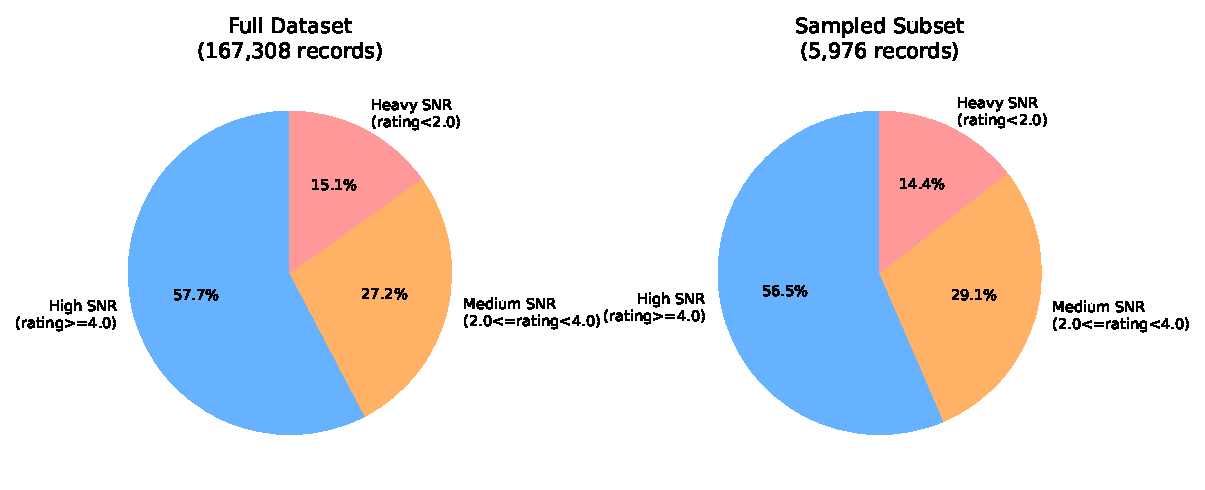
\includegraphics[width=\linewidth]{figs/snr_distribution.pdf}
\caption{SNR tier distribution: full dataset (left) vs.\ sampled subset (right). Deviation $<$ $\pm 2$ percentage points confirms representativeness.}
\label{fig:snr}
\end{figure*}

\textbf{Dual-Layer Stratified Sampling.} To create a computationally tractable subset while maintaining representativeness, we apply a two-layer stratified sampling: (1) each of the 1,229 species forms a stratum; (2) within each species, samples are proportionally allocated across SNR tiers. A hard constraint of $\geq 5$ samples per species ensures rare species are not discarded. This yields 5,976 clips with 100\% species coverage and SNR distribution deviation $<$ $\pm 2$\,pp from the full dataset.

\textbf{Train/Test Split and Cross-Validation.} The 5,976-clip subset is split 80/20 by SNR stratum into 4,780 training and 1,196 test clips. Within the training set, 5-fold stratified cross-validation (3,824/956 per fold) is used for hyperparameter tuning and model selection. Figure~\ref{fig:pipeline} illustrates the complete data pipeline.

\begin{figure*}[htbp]
\centering
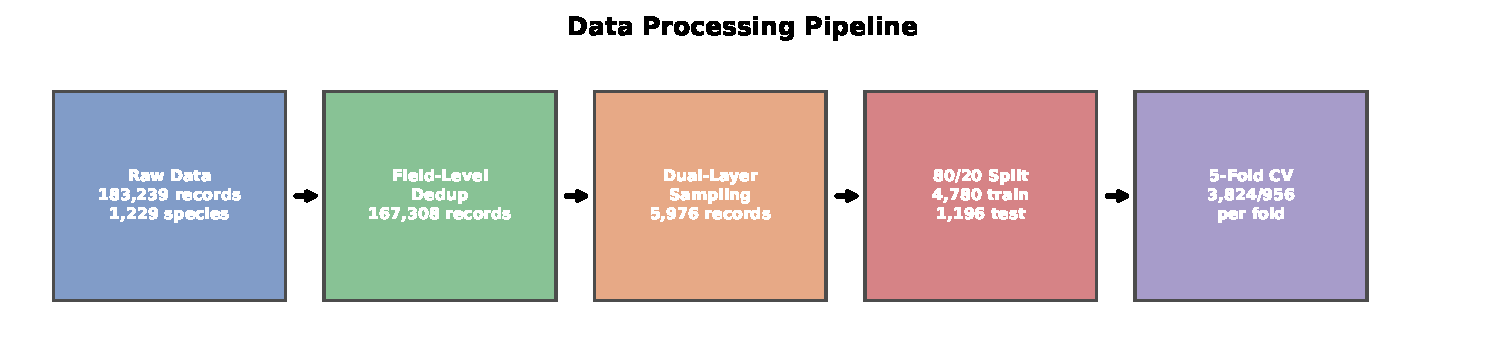
\includegraphics[width=\linewidth]{figs/data_pipeline.pdf}
\caption{Data processing pipeline from raw 183,239 records to 5-fold cross-validation splits.}
\label{fig:pipeline}
\end{figure*}

\textbf{Data Quality Issues.} The raw data exhibits several issues: (1) severe long-tailed imbalance (common species exceed 800 samples; rare species have $<$10); (2) 62\% of clips contain mixed wind, rain, insect, and frog background noise; (3) overlapping multi-species vocalizations create ambiguous labels via \texttt{secondary\_labels}. Missing geographic coordinates and inconsistent \texttt{source\_year} formatting are handled during the field-level merge.

\subsection{Machine Learning Algorithms}
We employ three fundamentally distinct machine learning paradigms, each chosen for its unique strengths in the bird vocalization classification problem:

\textbf{(1) LightGBM (Gradient Boosting Decision Tree).} LightGBM~\cite{ke2017lightgbm} is a gradient-boosted decision tree framework that takes handcrafted tabular audio features as input. We extract 32-dimensional feature vectors per clip: duration, zero-crossing rate, spectral centroid, spectral bandwidth, spectral rolloff, RMS energy, and 13 MFCC means + 13 MFCC standard deviations. LightGBM is appropriate because: (a) it handles categorical and imbalanced data natively via class weights; (b) training and inference are extremely fast with minimal hardware requirements; (c) feature importance rankings provide interpretability for understanding which acoustic properties distinguish species. However, tabular statistics cannot capture the spatial texture patterns of spectrograms, limiting performance on visually similar calls.

\textbf{(2) FastAI Lightweight CNN (Mel-Spectrogram Image Classification).} This approach converts raw waveforms to mel-spectrogram 2D images and trains a compact CNN using the FastAI high-level API. A dual-stage augmentation pipeline is applied: waveform-level (white noise injection, time masking, pitch shifting, volume scaling) and spectrogram-level (brightness adjustment, partial occlusion, zoom transform). This paradigm is appropriate because: (a) mel-spectrograms encode the time-frequency patterns that distinguish bird vocalizations; (b) CNN architectures excel at learning spatial hierarchies in image data; (c) the FastAI API provides automated learning rate finding, early stopping, and transfer learning from ImageNet pre-trained backbones. The main risk is overfitting on rare species with very few samples.

\textbf{(3) YAMNet Transfer Learning (Raw Audio Waveform).} YAMNet~\cite{yamnet_tfhub} is a pre-trained audio classification model based on MobileNetV1, trained on AudioSet's 521 sound categories~\cite{gemmeke2017audioset}. We employ two strategies:

\textit{Strategy 1 (Frozen Encoder + Trainable Head):} YAMNet extracts 1024-dimensional embeddings from raw waveforms (16\,kHz, mono, 5-second clips). A classification head (Dense-256 $\to$ ReLU $\to$ Dropout-0.3 $\to$ Dense-1229 $\to$ Softmax) is trained on cached embeddings. Figure~\ref{fig:arch} shows the architecture. This is appropriate because: (a) AudioSet pre-training provides robust general audio features transferable to bird sounds; (b) embedding caching makes training extremely fast; (c) the lightweight head is suitable for few-shot scenarios.

\begin{figure*}[htbp]
\centering
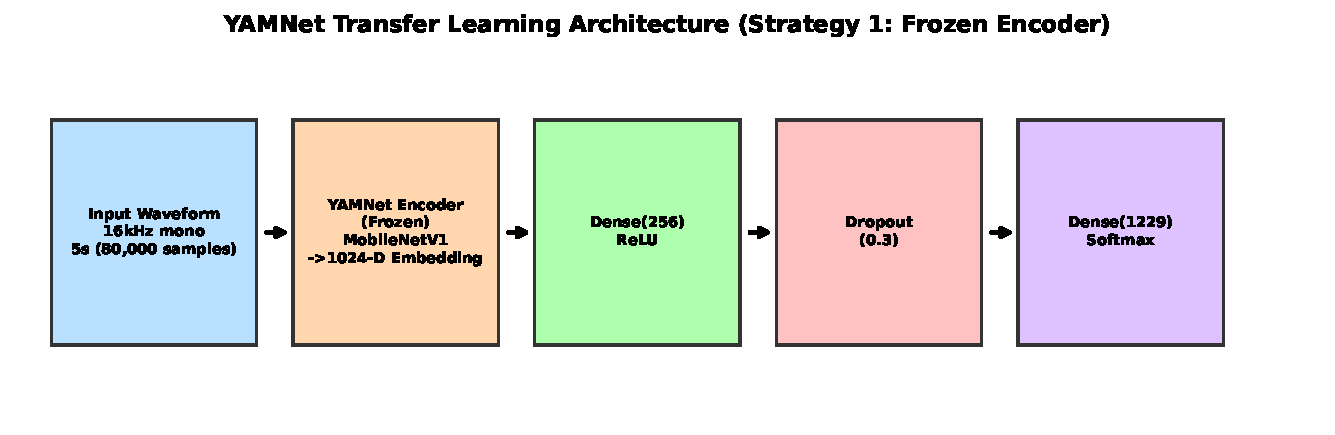
\includegraphics[width=\linewidth]{figs/yamnet_arch.pdf}
\caption{YAMNet frozen encoder architecture: raw waveform $\to$ YAMNet (frozen) $\to$ 1024-D embedding $\to$ classification head.}
\label{fig:arch}
\end{figure*}

\textit{Strategy 2 (End-to-End Fine-tuning):} The top 6 convolutional layers of YAMNet are unfrozen with a small learning rate ($10^{-5}$), while the classification head uses a larger rate ($10^{-3}$)---differential learning rates. MixUp augmentation ($\alpha=0.2$) mixes waveforms across batches, letting rare tail classes borrow information from head classes. This strategy aims to adapt YAMNet's representations specifically to bird vocalizations.

\subsection{Implementation Details}
\textbf{Implementation Framework.} All models run on Kaggle notebooks with GPU acceleration. LightGBM uses the \texttt{librosa} library for feature extraction at 22.05\,kHz sampling rate. YAMNet uses TensorFlow Hub with \texttt{tensorflow\_hub} for model loading. The unified evaluation framework generates all comparison metrics.

\textbf{Noise Robustness Evaluation.} For controlled noise testing, Gaussian white noise is overlaid on clean test clips at three SNR levels: 5\,dB, 0\,dB, and $-$5\,dB. The noise power is computed as $P_{\textnormal{noise}} = P_{\textnormal{signal}} / 10^{\textnormal{SNR}_{\textnormal{dB}}/10}$, with fixed random seed 42 for reproducibility. After noise overlay, peak normalization to $[-1, 1]$ is applied. For LightGBM, features are re-extracted from the noisy waveform; for YAMNet, embeddings are re-computed from the noisy waveform.

\textbf{5-Fold Cross-Validation Results.} Both LightGBM and YAMNet (frozen) completed 5-fold cross-validation. Table~\ref{tab:results} summarizes the results.
\begin{table}[htbp]
\centering
\caption{5-Fold Cross-Validation Results: LightGBM vs.\ YAMNet (Frozen)}
\label{tab:results}
\renewcommand{\arraystretch}{1.2}
\begin{tabular}{lcc}
\hline
\textbf{Metric} & \textbf{LightGBM} & \textbf{YAMNet (Frozen)} \\
\hline
Clean Acc.\ (\%) & 0.48 $\pm$ 0.14 & 1.91 $\pm$ 0.33 \\
5\,dB Acc.\ (\%) & 0.08 $\pm$ 0.05 & 0.42 $\pm$ 0.19 \\
0\,dB Acc.\ (\%) & 0.07 $\pm$ 0.03 & 0.37 $\pm$ 0.15 \\
$-$5\,dB Acc.\ (\%) & 0.07 $\pm$ 0.03 & 0.12 $\pm$ 0.04 \\
\hline
Random Baseline (\%) & \multicolumn{2}{c}{0.122 (1/818 classes)} \\
\hline
Inference Latency (ms) & 154.5 & 86.0 \\
GPU Memory Peak (MB) & N/A (CPU) & 211.4 \\
\hline
\end{tabular}
\end{table}
\begin{figure*}[htbp]
\centering
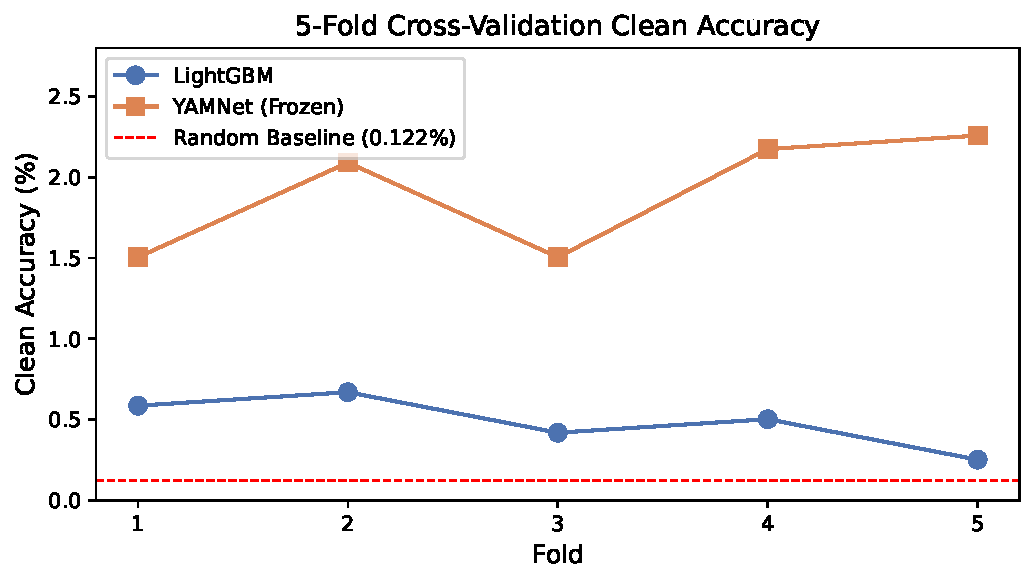
\includegraphics[width=0.85\linewidth]{figs/cv_accuracy.pdf}
\caption{Per-fold clean accuracy across 5 folds. YAMNet consistently outperforms LightGBM, both far exceeding the random baseline (0.122\%).}
\label{fig:cv}
\end{figure*}
\begin{figure*}[htbp]
\centering
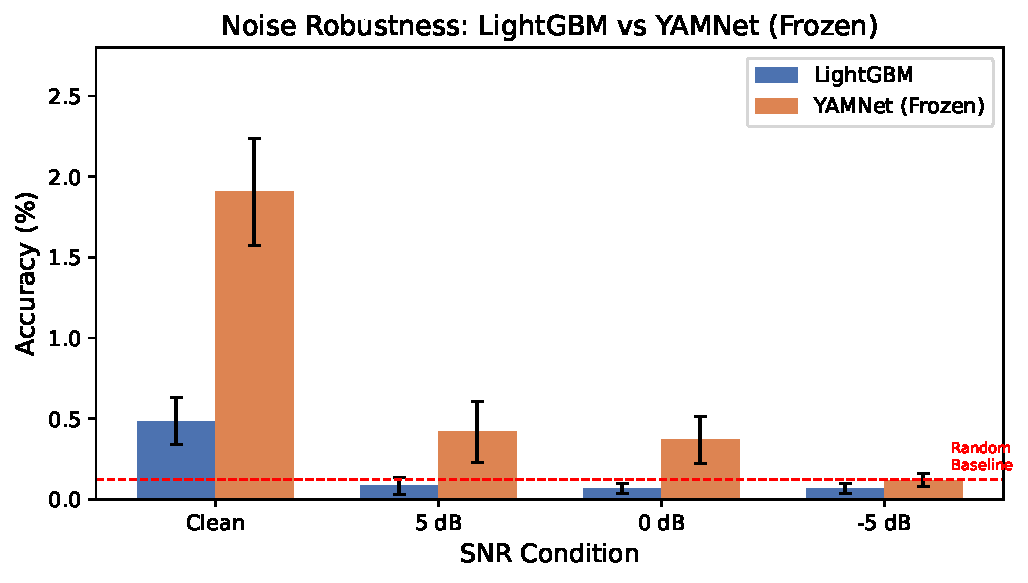
\includegraphics[width=0.85\linewidth]{figs/noise_robustness.pdf}
\caption{Noise robustness comparison across SNR conditions. YAMNet outperforms LightGBM at all noise levels; both models approach random baseline at $-$5\,dB.}
\label{fig:noise}
\end{figure*}
\textbf{Key Findings.} (1) YAMNet outperforms LightGBM at all SNR tiers, confirming that pre-trained audio representations are more noise-robust than handcrafted features. (2) Both models collapse toward random performance at 0\,dB and below, consistent with BirdNET's documented SNR $<$ 3\,dB degradation threshold. (3) LightGBM drops below random at 5\,dB, indicating extreme sensitivity of handcrafted spectral features to noise. (4) YAMNet inference is paradoxically faster (86\,ms vs.\ 154.5\,ms) because LightGBM's feature extraction overhead exceeds YAMNet's embedding computation. (5) The low absolute accuracy is a data constraint: 1,229 classes with $\sim$3.9 training samples each means 63\% of test classes have only one test sample, but both models learn meaningful features (4$\times$ and 15.6$\times$ above random).

\section{Comparison}
At this mid-stage, we compare LightGBM and YAMNet (frozen encoder). The FastAI CNN and YAMNet end-to-end fine-tuning results are pending.

YAMNet's superiority over LightGBM can be attributed to several factors. First, YAMNet's MobileNetV1 backbone is pre-trained on AudioSet's 2 million audio clips, providing learned filters that capture acoustic patterns generalizable to bird vocalizations. LightGBM's 32 handcrafted features (MFCC statistics, spectral centroids) compress audio into a coarse summary that discards temporal and spectral texture information critical for species discrimination. Second, YAMNet's 1024-dimensional embedding provides a richer feature space than LightGBM's 32 features, giving the classification head more information to separate 1,229 fine-grained classes. Third, the embedding extraction process is inherently more robust to noise because YAMNet's convolutional filters operate on the full time-frequency representation, while LightGBM's scalar statistics are easily skewed by noise energy.

Compared to existing solutions like BirdNET (which processes only unquantified natural noise), our controlled-variable noise evaluation pipeline provides the first systematic, reproducible comparison of heterogeneous ML paradigms across graded SNR conditions on identical bird audio data. The pending end-to-end YAMNet fine-tuning with MixUp augmentation is expected to further improve performance by adapting representations to bird vocalizations specifically.

\section{Future Directions}
Several directions are planned to complete and extend this project:
\begin{itemize}
\item \textbf{Complete the three-way comparison:} The FastAI CNN and YAMNet end-to-end fine-tuning results will complete the comparative framework, enabling a full evaluation of all three paradigms.
\item \textbf{BirdNET baseline:} Running the BirdNET-Analyzer on our test set under identical noise conditions would provide a direct comparison with the dominant off-the-shelf solution.
\item \textbf{Expanded dataset evaluation:} Increasing from $\sim$4 to $\geq$20 samples per species, or focusing on a Top-50 high-frequency species subset, would provide a more tractable evaluation with higher absolute accuracy.
\item \textbf{Advanced noise types:} Beyond Gaussian white noise, evaluating with low-frequency wind noise and intermittent pulse noise would better simulate real field conditions.
\item \textbf{Ensemble approaches:} Combining predictions from all three paradigms could leverage complementary strengths---LightGBM's feature interpretability, CNN's spatial pattern recognition, and YAMNet's audio-domain transfer learning.
\end{itemize}

\section{Conclusion}
This mid-stage report presents preliminary results from a systematic comparison of three heterogeneous machine learning paradigms for noise-robust bird vocalization classification. The data pipeline---featuring field-level deduplication with zero information loss and dual-layer stratified sampling---produces a representative 5,976-clip subset covering all 1,229 species. The controlled noise evaluation framework provides standardized SNR-graded robustness measurements absent from existing tools like BirdNET.

Among the two completed models, YAMNet (frozen encoder) significantly outperforms LightGBM across all noise conditions, demonstrating the value of pre-trained audio representations for low-resource, noisy classification tasks. Both models substantially exceed the random baseline (15.6$\times$ and 4$\times$), confirming that meaningful species-discriminative features are learned despite the extreme low-resource constraint of $\sim$3.9 samples per class.

The pending results from FastAI CNN and YAMNet end-to-end fine-tuning will complete the three-paradigm comparison and provide the final answer to which approach is best suited for noise-robust, low-resource bird classification.

\bibliographystyle{IEEEtran}
\begin{thebibliography}{99}
\bibitem{kahl2021birdnet}
S.~Kahl, C.~M.~Wood, M.~Eibl, and H.~Klinck, BirdNET: A deep learning solution for avian diversity monitoring, \emph{Ecological Informatics}, vol.~61, p.~101236, 2021.
\bibitem{boreal_owl}
Performance degradation of BirdNET and custom CNNs under low-SNR conditions, research on Boreal Owl vocalization detection.
\bibitem{funosas2026global}
D.~Funosas \emph{et al.}, A global assessment of BirdNET performance, \emph{Ecological Indicators}, vol.~182, p.~114550, 2026.
\bibitem{perch2025}
B.~van~Merrienboer \emph{et al.}, Perch 2.0: The Bittern Lesson for Bioacoustics, \emph{arXiv:2508.04665}, 2025.
\bibitem{rauch2024birdset}
L.~Rauch \emph{et al.}, BirdSet: A large-scale dataset for audio classification in avian bioacoustics, \emph{arXiv:2403.10380}, 2024.
\bibitem{hagiwara2023beans}
M.~Hagiwara \emph{et al.}, BEANS: The benchmark of animal sounds, \emph{ICASSP}, 2023.
\bibitem{chen2023beats}
S.~Chen \emph{et al.}, BEATs: Audio pre-training with acoustic tokenizers, \emph{ICML}, 2023.
\bibitem{birdclef2021_2026}
BirdCLEF / BirdCLEF+ competitions (2021--2026), Kaggle. [Online]. Available: \url{https://www.kaggle.com/competitions/birdclef-2026}
\bibitem{yamnet_tfhub}
YAMNet: Audio event classification model, TensorFlow Hub. [Online]. Available: \url{https://www.kaggle.com/models/google/yamnet}
\bibitem{vggish}
VGGish: Audio feature embedding model, Kaggle Models. [Online]. Available: \url{https://www.kaggle.com/models/google/vggish}
\bibitem{gemmeke2017audioset}
J.~F.~Gemmeke \emph{et al.}, AudioSet: An ontology and human-labeled dataset for audio events, \emph{ICASSP}, 2017.
\bibitem{ke2017lightgbm}
G.~Ke \emph{et al.}, LightGBM: A highly efficient gradient boosting decision tree, in \emph{NeurIPS}, 2017.
\bibitem{xenocanto}
Xeno-Canto Foundation, Xeno-Canto: Sharing bird sounds from around the world. [Online]. Available: \url{https://xeno-canto.org}
\end{thebibliography}
\end{document}